\documentclass[aspectratio=169,11pt]{beamer}
\usetheme[progressbar=frametitle]{metropolis}
\usepackage[sfdefault]{FiraSans}
\usepackage{booktabs}
\usepackage{amsmath}
\usepackage{pgfplots}
\pgfplotsset{compat=1.18}
\graphicspath{{../figures/}}

\definecolor{prey}{HTML}{D62728}
\definecolor{pred}{HTML}{1F77B4}
\newcommand{\hl}[1]{\textbf{\color{prey}#1}}

\title{Predatory Trading}
\subtitle{Replicating, verifying and extending Brunnermeier \& Pedersen (2005)}
\author{Harsh Gupta \quad (22IM3FP29)}
\institute{Market Microstructure \quad$\cdot$\quad Prof.\ Ajay Kumar Mishra\\
  Indian Institute of Technology Kharagpur}
\date{}

\begin{document}

\maketitle

% ---------------------------------------------------------------- 2
\begin{frame}{Why this matters}
  \begin{quote}
    ``\dots if lenders know that a hedge fund needs to sell something quickly,
    they will sell the same asset --- driving the price down even faster.
    Goldman, Sachs \& Co.\ and other counterparties to LTCM did exactly that in 1998.''
  \end{quote}
  \hfill --- \emph{Business Week}, 2001 (quoted in the paper, Table I)

  \vspace{1em}
  \begin{itemize}
    \item 1987 crash: traders sold \emph{ahead of} portfolio insurers (Brady Report)
    \item Fed on LTCM: unwinding could cause ``large losses, or worse'' for others
  \end{itemize}
\end{frame}

% ---------------------------------------------------------------- 3
\begin{frame}{The idea in one picture}
  \begin{columns}[c]
    \column{0.55\textwidth}
    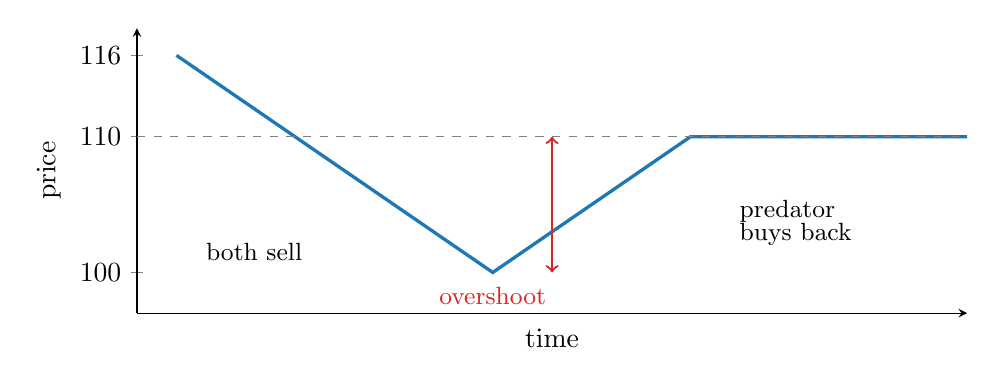
\begin{tikzpicture}
      \begin{axis}[width=\linewidth, height=5.2cm, xmin=4.9, xmax=7, ymin=97, ymax=118,
                   xlabel={time}, ylabel={price}, axis lines=left, xtick=\empty, ytick={100,110,116}]
        \addplot[very thick, pred] coordinates {(5,116) (5.8,100) (6.3,110) (7,110)};
        \addplot[dashed, gray] coordinates {(4.9,110) (7,110)};
        \node[prey, font=\small] at (axis cs:5.8,98.3) {overshoot};
        \draw[<->, prey, thick] (axis cs:5.95,100) -- (axis cs:5.95,110);
        \node[font=\small, anchor=west] at (axis cs:5.05,101.5) {both sell};
        \node[font=\small, anchor=west] at (axis cs:6.4,104.5) {predator};
        \node[font=\small, anchor=west] at (axis cs:6.4,102.8) {buys back};
      \end{axis}
    \end{tikzpicture}
    \column{0.45\textwidth}
    \begin{itemize}
      \item A large trader is \hl{forced to sell}
      \item Rivals know it --- and \hl{sell too}
      \item Price falls \emph{below} its new level
      \item Rivals \hl{buy back} at the bottom
    \end{itemize}
    \vspace{0.6em}
    Victim's extra loss $=$ predators' profit.\\
    Liquidity vanishes \emph{when it is needed most}.
  \end{columns}
\end{frame}

% ---------------------------------------------------------------- 4
\begin{frame}{The model}
  \small
  \begin{tabular}{@{}p{0.17\textwidth}p{0.45\textwidth}l@{}}
    \toprule
    Ingredient & Meaning & Formula \\
    \midrule
    Demand curve & selling to ordinary investors lowers the price & $p(t) = \mu - \lambda\,(S - X(t))$ \\
    Limited capital & each big trader holds at most $\bar x$ & $|x_i| \le \bar x$ \\
    Speed limit & big traders together trade $\le A$ per unit time & $\bigl|\sum_i a_i\bigr| \le A$ \\
    Distress at $t_0$ & $I_d$ traders must sell at speed $A/I$ & $I_p = I - I_d$ predators \\
    \bottomrule
  \end{tabular}

  \normalsize
  \vspace{1em}
  \begin{itemize}
    \item $X$ = total holdings of the big traders; $\lambda$ = price impact
    \item Everyone knows who is distressed; predators maximise expected profit
    \item Paper's example: $S = 40$, $\mu = 140$, $\lambda = 1$, $A = 20$, $\bar x = 10$, $x(t_0) = 8$
  \end{itemize}
\end{frame}

% ---------------------------------------------------------------- 5
\begin{frame}{The key insight (Lemma 1)}
  A predator's problem reduces to
  \[
    \min_{a_i} \int_0^T a_i(t)\, X_{-i}(t)\, dt
    \quad\text{s.t. } x_i(T) = \bar x
  \]
  where $X_{-i}$ is \hl{everyone else's} holdings.

  \vspace{0.8em}
  \begin{itemize}
    \item Its \emph{own} price impact cancels out (paid when buying, earned back when selling)
    \item So: \hl{sell while $X_{-i}$ is falling}, \hl{buy once it stops}
    \item Profit comes from the \emph{victim's} price impact $\Rightarrow$ predation, not manipulation
  \end{itemize}

  \vspace{0.6em}
  \alert{For us:} the objective is \emph{linear} in the predator's trades $\Rightarrow$ best responses
  are linear programs (slide~\ref{lp}).
\end{frame}

% ---------------------------------------------------------------- 6
\begin{frame}{One predator (Prop.~1): our simulation}
  \begin{columns}[c]
    \column{0.5\textwidth}
    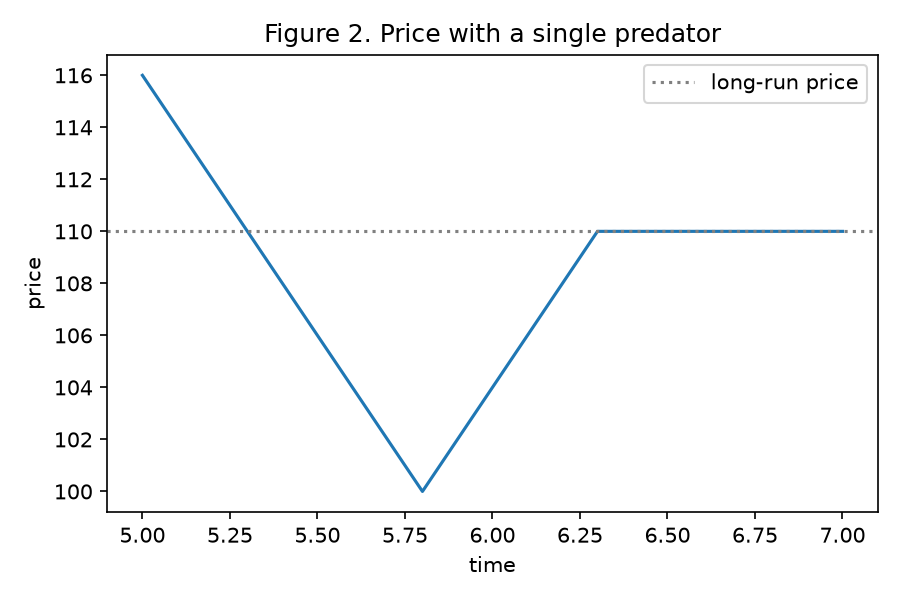
\includegraphics[width=\linewidth]{fig2_price.png}
    \column{0.5\textwidth}
    \begin{itemize}
      \item $t = 5 \to 5.8$: both sell 8 shares; 16 sold $\Rightarrow$ $116 \to \mathbf{100}$
      \item $t = 5.8 \to 6.3$: predator buys back to 10 $\Rightarrow$ $\mathbf{110}$
      \item Overshoot of \hl{10}
    \end{itemize}
    \vspace{0.5em}
    \textbf{Why sell below 110?} The last share sells at $\approx 101$ and is bought back at
    $\approx 100.5$: \hl{+0.50}. Our simulation reproduces this to the cent.
  \end{columns}
\end{frame}

% ---------------------------------------------------------------- 7
\begin{frame}[standout]
  Live demo\\[0.5em]
  \normalsize\texttt{uv run streamlit run app.py}\\[0.5em]
  ``Single predator'' $\rightarrow$ ``Many predators''
\end{frame}

% ---------------------------------------------------------------- 8
\begin{frame}{Competition, and what a position is worth}
  \begin{columns}[t]
    \column{0.5\textwidth}
    \centering
    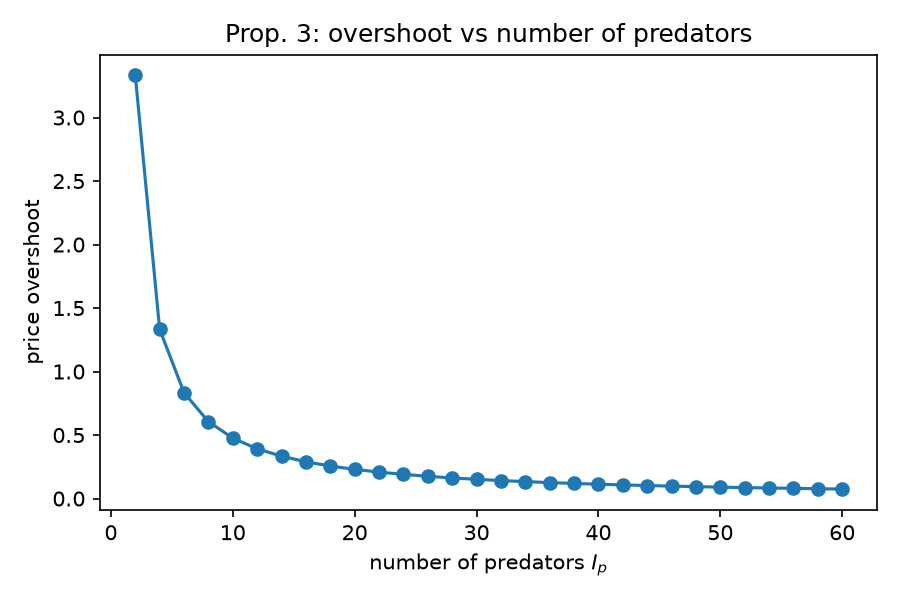
\includegraphics[width=0.95\linewidth]{prop3_overshoot.png}\\
    \small \textbf{Prop.~3:} predators race to rebuild first $\Rightarrow$
    overshoot $3.33 \to 0.83 \to 0.26$ for $2, 6, 18$ predators
    \column{0.5\textwidth}
    \centering
    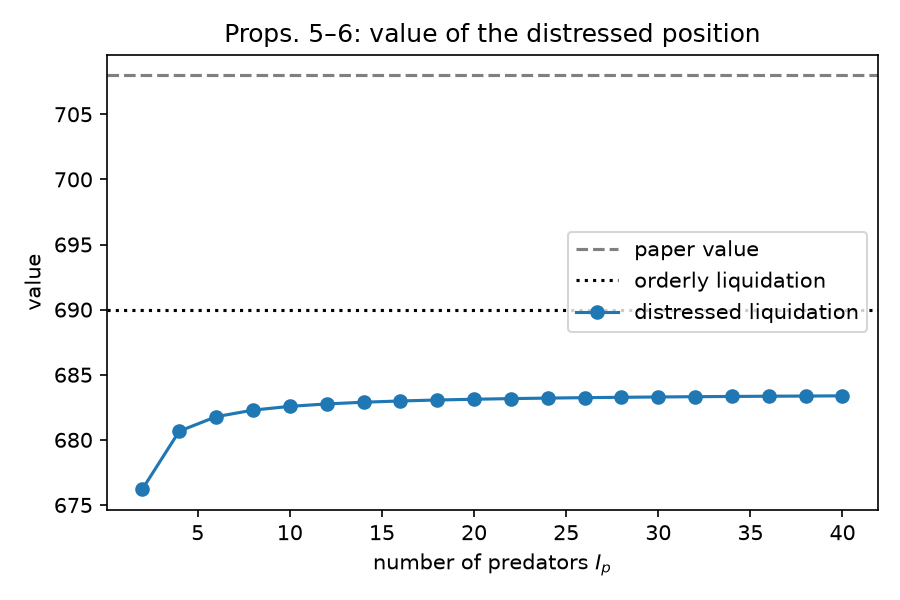
\includegraphics[width=0.95\linewidth]{prop56_valuation.png}\\
    \small \textbf{Props.~5--6:} paper $708 >$ orderly $690 >$ distressed
    $676.2 \to 683.4$, even as predator competition increases
  \end{columns}
\end{frame}

% ---------------------------------------------------------------- 9
\begin{frame}{Market design (Props.~8--9)}
  \begin{columns}[c]
    \column{0.58\textwidth}
    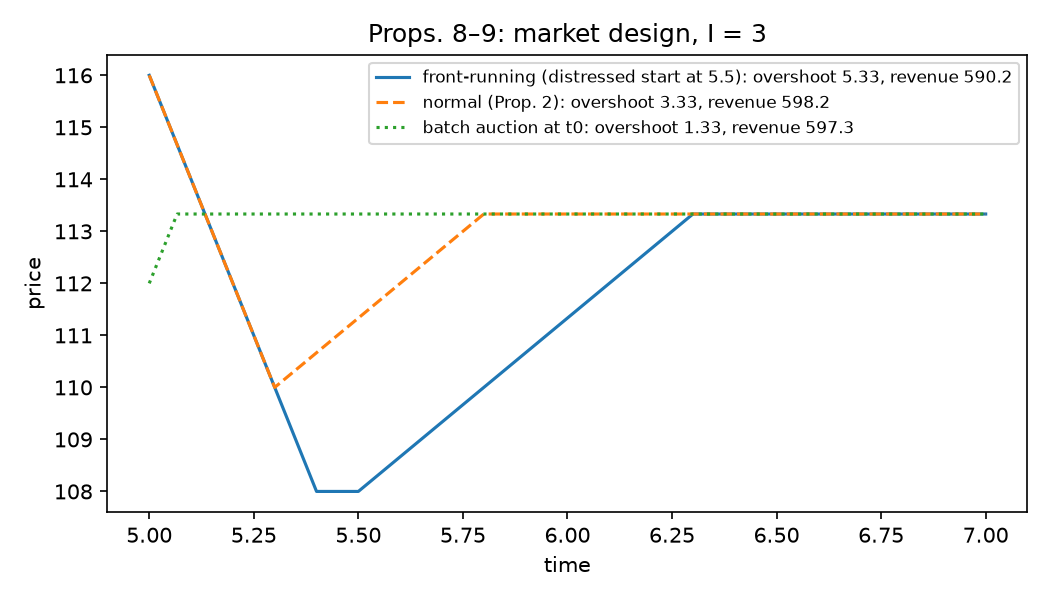
\includegraphics[width=\linewidth]{prop89_market_design.png}
    \column{0.42\textwidth}
    \small
    \begin{tabular}{@{}lrr@{}}
      \toprule
      Market & Overshoot & Seller gets \\
      \midrule
      Front-running & 5.33 & 590.2 \\
      Normal & 3.33 & 598.2 \\
      Batch auction & 1.33 & 597.3 \\
      \bottomrule
    \end{tabular}

    \vspace{0.8em}
    \normalsize
    \alert{Our finding:} a batch auction (circuit breaker) calms the price, but does
    \hl{not} raise the seller's revenue --- everything sells at one price.
  \end{columns}
\end{frame}

% ---------------------------------------------------------------- 10
\begin{frame}{Does it hold up? (1) Best response as a linear program}
  \label{lp}
  Fix everyone else at the paper's strategy; let a solver find one predator's
  \emph{best possible} strategy.

  \vspace{0.6em}
  \centering
  \begin{tabular}{@{}lrr@{}}
    \toprule
    Case & Paper's strategy pays & Best possible pays \\
    \midrule
    Prop.~1 (one predator) & 1214.000000 & 1214.000000 \\
    Prop.~2, $I = 3$ & 787.111111 & 787.111111 \\
    Prop.~2, $I = 9$ & 261.444444 & 261.444444 \\
    Prop.~2$'$ (spare capital) & 702.000000 & 702.000000 \\
    Prop.~8 (front-running) & 791.111111 & 791.111111 \\
    \bottomrule
  \end{tabular}

  \vspace{0.6em}
  \raggedright
  \hl{No profitable deviation} $\Rightarrow$ the paper's strategies are equilibria.
  Sensitivity check: without the speed limit the solver earns 1324, so the test can fail.
\end{frame}

% ---------------------------------------------------------------- 11
\begin{frame}{Does it hold up? (2) Traders learn to prey}
  \centering
  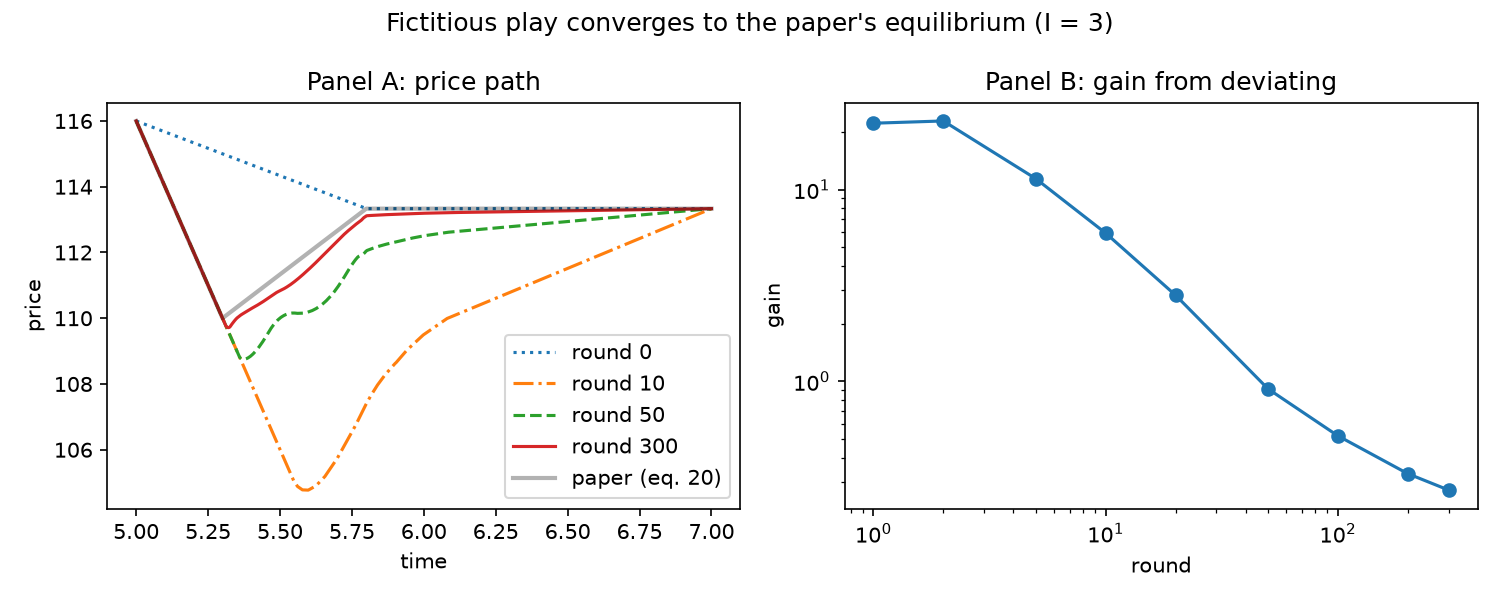
\includegraphics[width=0.85\linewidth]{fictitious_play.png}

  \raggedright
  \small
  Start: predators just buy (no predation). Each round they move a step toward their best
  response (fictitious play). Round 10: they \hl{overdo it} (price $\approx 105$). Round 300:
  the paper's path. Gain from deviating $22 \to 0.27$.
  \quad\alert{Predation is not assumed --- it is learned.}
\end{frame}

% ---------------------------------------------------------------- 12
\begin{frame}{Extension: collusion}
  \centering
  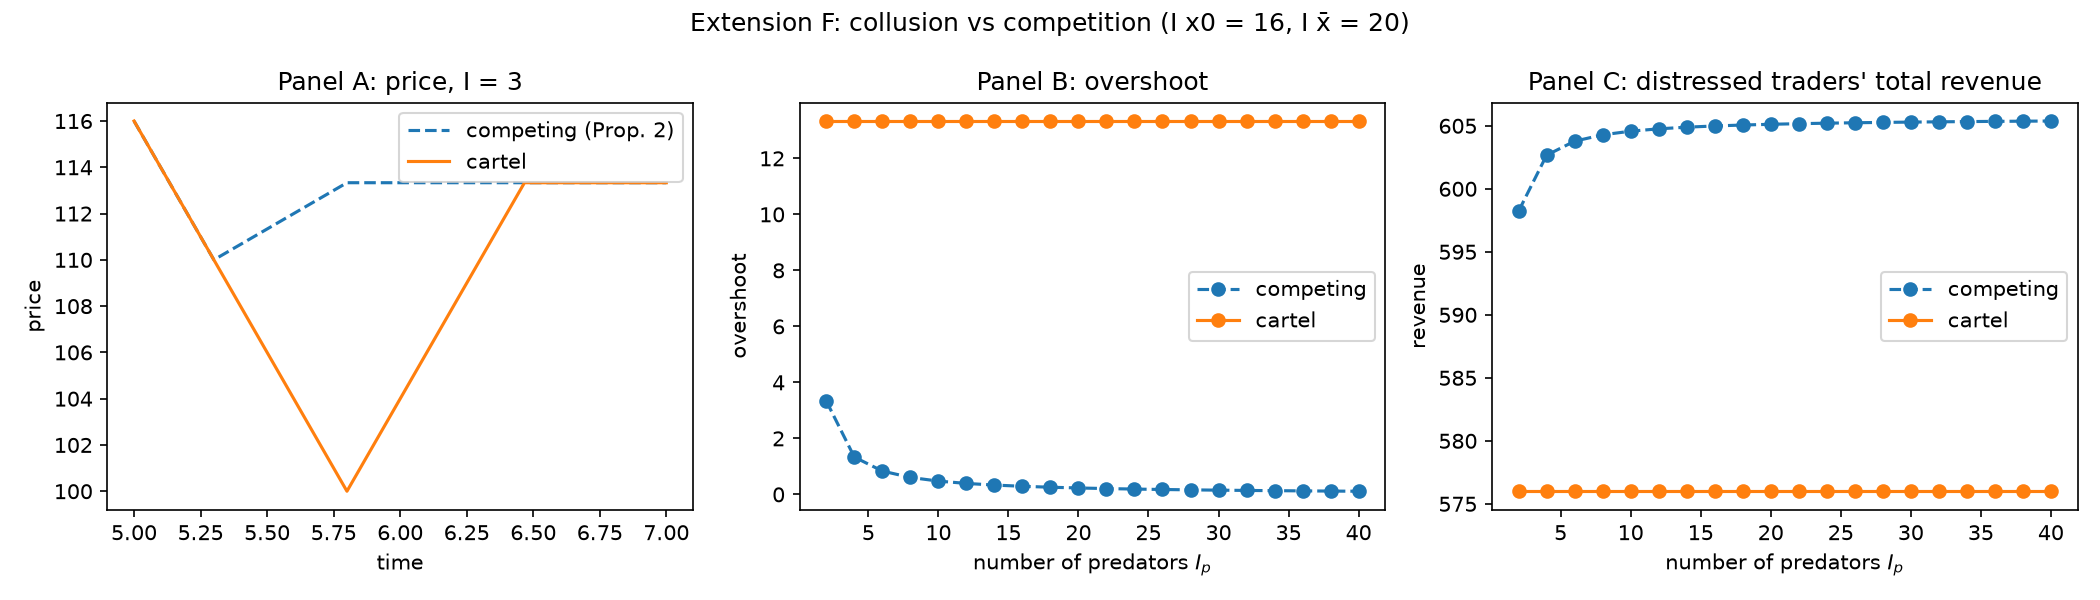
\includegraphics[width=0.95\linewidth]{collusion.png}

  \raggedright
  \small
  \begin{itemize}
    \item A cartel acts as one big predator: overshoot \hl{13.33} vs 3.33, and it does not shrink with size
    \item A \emph{pure transfer}: predators gain exactly what the victims lose
    \item \alert{Unstable:} a member gains 16.67 by cheating (2.1\% of its profit; 4.3\% with 6 members)
  \end{itemize}
\end{frame}

% ---------------------------------------------------------------- 13
\begin{frame}{Extension: contagion}
  \centering
  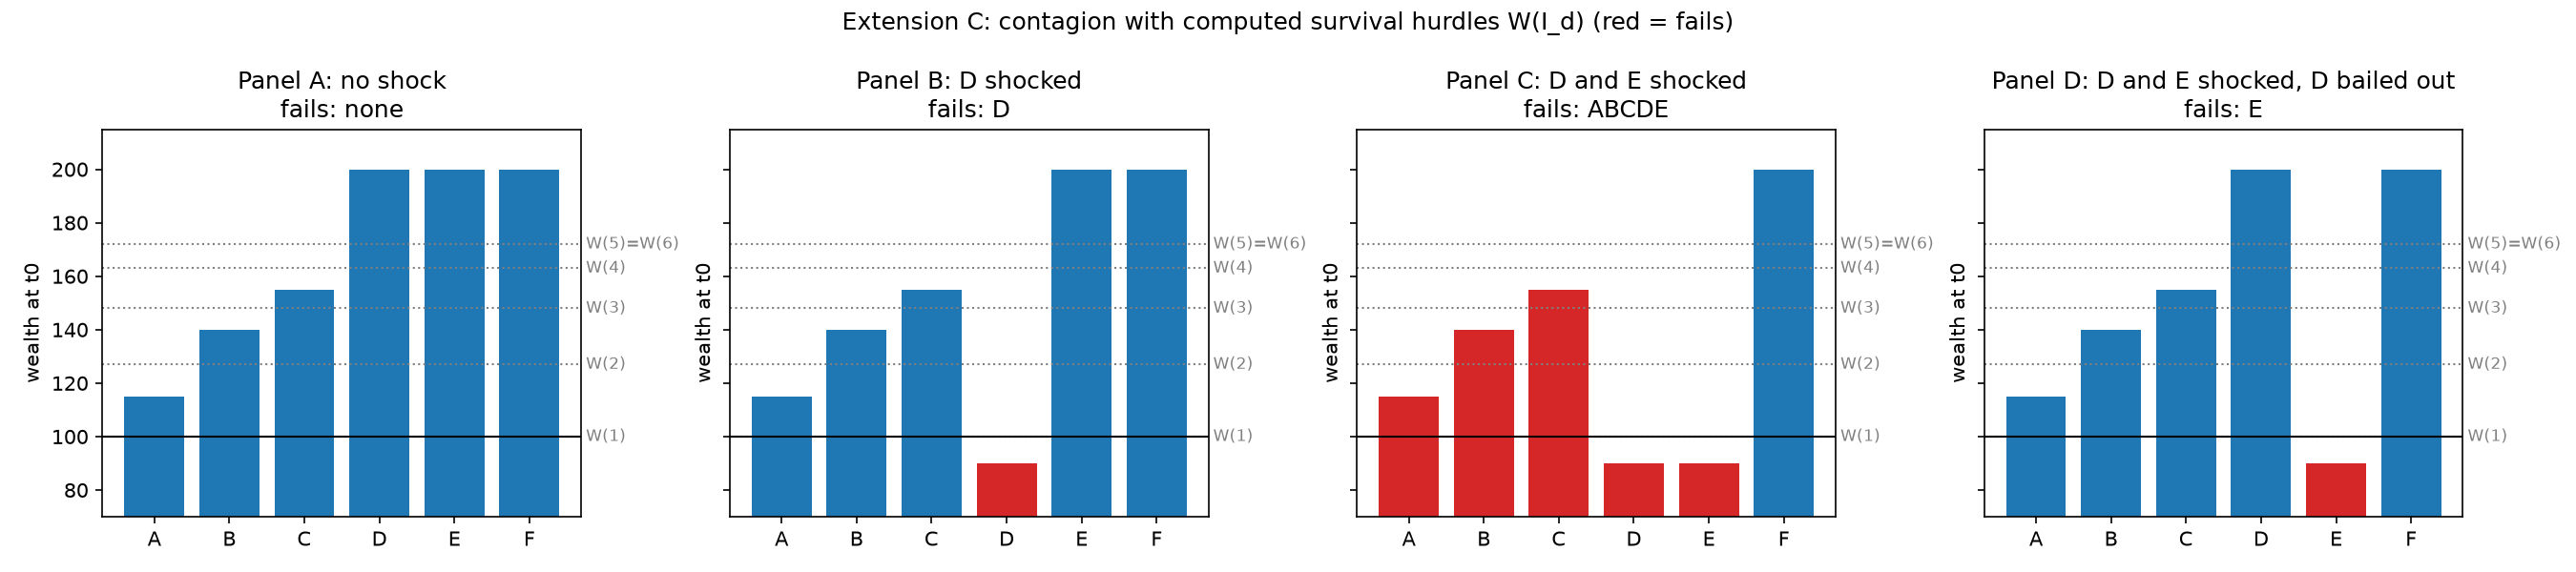
\includegraphics[width=0.95\linewidth]{contagion.png}

  \raggedright
  \small
  \begin{itemize}
    \item We \emph{computed} the paper's survival hurdles $W(I_d)$ (eq.~21) by sequential linear programming: $W = 100, 127, 148, 163, 172, 172$
    \item Best way to survive: sell, then \hl{buy at the bottom} to prop up your own paper wealth
    \item D and E shocked $\Rightarrow$ ripple \hl{D, E $\to$ A $\to$ B $\to$ C}; bailing out D stops it
  \end{itemize}
\end{frame}

\begin{frame}[standout]
  Live demo\\[0.5em]
  \normalsize ``Contagion'' page: shock D and E, then bail out D
\end{frame}

% ---------------------------------------------------------------- 14
\begin{frame}{Extension: predators with unequal positions}
  \begin{columns}[c]
    \column{0.6\textwidth}
    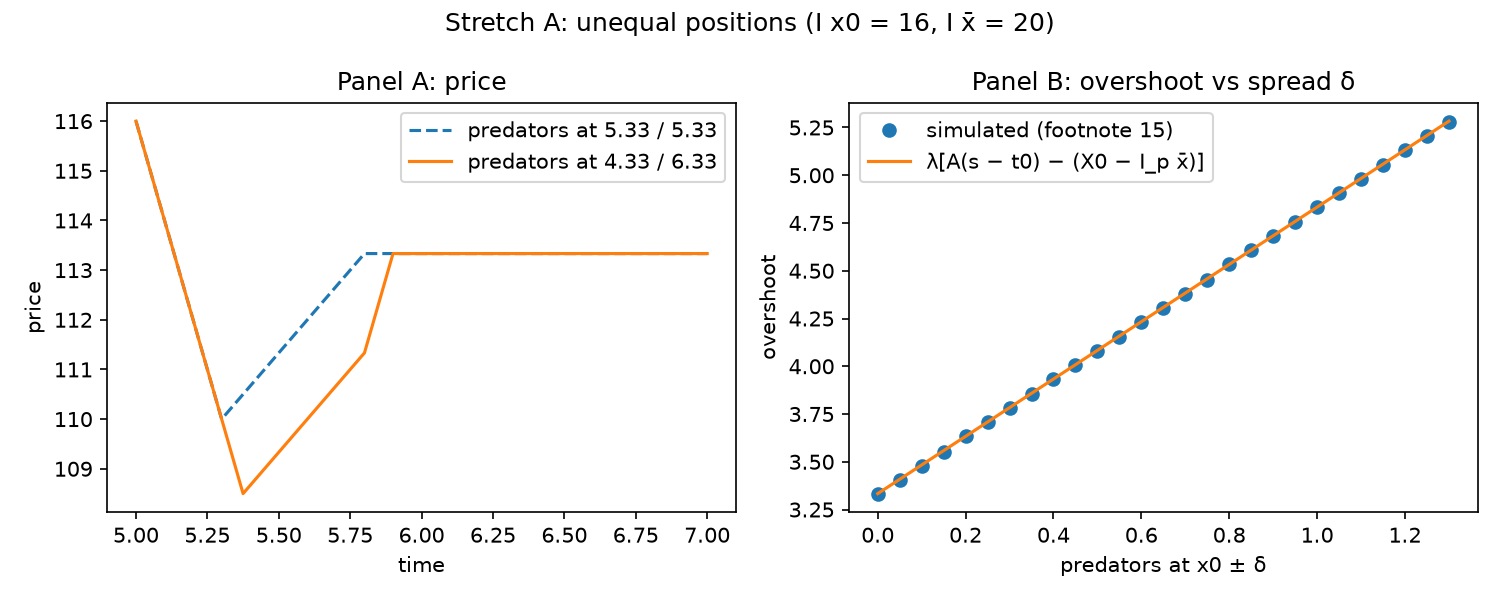
\includegraphics[width=\linewidth]{unequal_positions.png}
    \column{0.4\textwidth}
    \small
    Paper (footnote 15, no proof): more dispersed holdings $\Rightarrow$ more overshoot.

    \vspace{0.5em}
    We confirm the footnote's equilibrium with the solver, and sharpen the claim:
    \[
      \text{overshoot} = \lambda\,[A(s - t_0) - (X_0 - I_p \bar x)]
    \]
    $s$ depends only on the \hl{smallest} predator: it keeps selling longest, and
    everyone sells with it.
  \end{columns}
\end{frame}

% ---------------------------------------------------------------- 15
\begin{frame}{Takeaways}
  \begin{columns}[t]
    \column{0.5\textwidth}
    \textbf{Economics}
    \begin{itemize}
      \item Liquidity disappears when it is needed most
      \item Secrecy protects funds (disclosure invites predation)
      \item Circuit breakers calm prices; bailouts stop cascades
      \item Collusion makes predation far worse --- but is unstable
    \end{itemize}
    \column{0.5\textwidth}
    \textbf{What we added}
    \begin{itemize}
      \item Exact simulator reproducing Props.~1--9 and Figs.~1--3
      \item Independent check: no profitable deviation (LP), and traders \emph{learn} the equilibrium
      \item New results on collusion, contagion and unequal positions
      \item Interactive app for every result
    \end{itemize}
  \end{columns}

  \vspace{1em}
  \centering
  \small 115 automated tests $\cdot$ \texttt{github.com/dudegladiator/predatory-trading}
\end{frame}

\begin{frame}[standout]
  Thank you\\[0.3em]
  \normalsize Questions?
\end{frame}

% ---------------------------------------------------------------- backup
\appendix

\begin{frame}{Backup: spare capital and disclosure (Props.~2$'$, 7)}
  \begin{columns}[c]
    \column{0.5\textwidth}
    \textbf{Prop.~2$'$:} if $x(t_0) < \frac{I_p - 1}{I - 1}\,\bar x$, competition to buy
    beats the urge to prey: predators buy at once, no overshoot.

    \vspace{0.5em}
    \textbf{Prop.~7:} traders build positions large enough that predation happens with
    positive probability. Disclosure shrinks positions ($9.0 \to 8.75$ for $I = 5$,
    $\pi = 0.5$) --- but never below the predation threshold.
    \column{0.5\textwidth}
    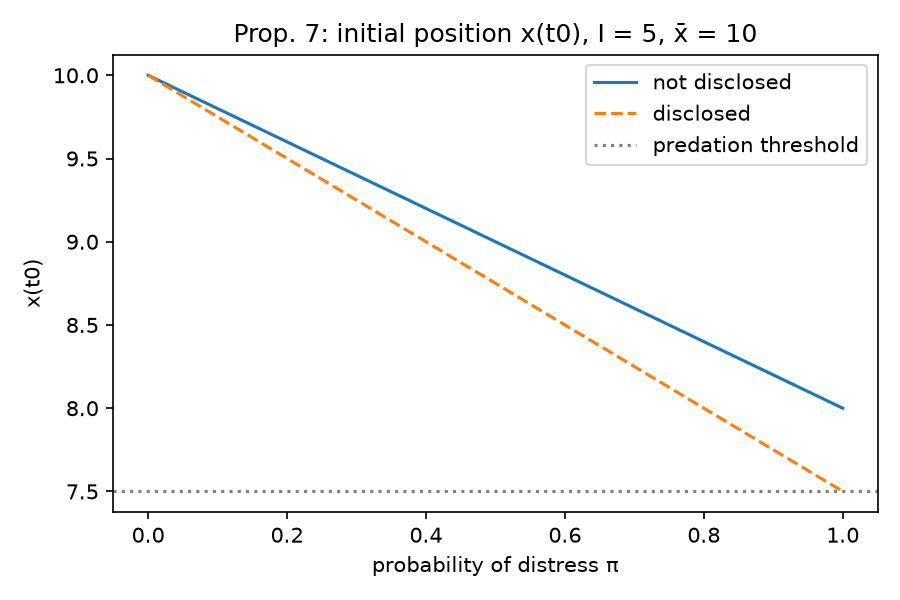
\includegraphics[width=\linewidth]{prop7_disclosure.png}
  \end{columns}
\end{frame}

\begin{frame}{Backup: how the simulation stays exact}
  \begin{itemize}
    \item Time grid $t_0, t_0 + dt, \dots, T$; trading rates constant within a step
    \item Price is linear in holdings $\Rightarrow$ linear within a step $\Rightarrow$
          cash $= -\sum a_k\,dt\,(p_k + p_{k+1})/2$ is \hl{exact}
    \item Switch times between grid points: rates averaged over the step
    \item Trading faster than the speed caps (eqs.~8--10) is charged $\gamma = \lambda I \bar x$
          per excess share --- added after we caught averaged learning strategies breaking the limit
  \end{itemize}
\end{frame}

\begin{frame}{Backup: computing the survival hurdle}
  \[
    W(I_d) = \underline W + D(I_d), \qquad
    D(I_d) = -\max_{a_i}\, \min_{t}\, \Delta W_i(t)
  \]
  \[
    \Delta W_i(t) = \lambda\Bigl[\tfrac12 (x_t^2 - x_0^2) + \textstyle\sum_{k<t} \bar x_k\, \Delta X_{-i,k}\Bigr]
  \]
  \begin{itemize}
    \item $x^2$ makes max--min non-convex $\Rightarrow$ replace $\tfrac12 x^2$ by its tangent
          (never above it), solve the LP, re-linearise, repeat
    \item Several starting paths; 25 random starts all reach the same values
    \item Identical at $dt = 0.005, 0.0025, 0.001$ $\Rightarrow$ no grid artifact
  \end{itemize}
\end{frame}

\end{document}
